\documentclass[tikz,border=5pt]{standalone}
\usepackage{tikz}

\begin{document}
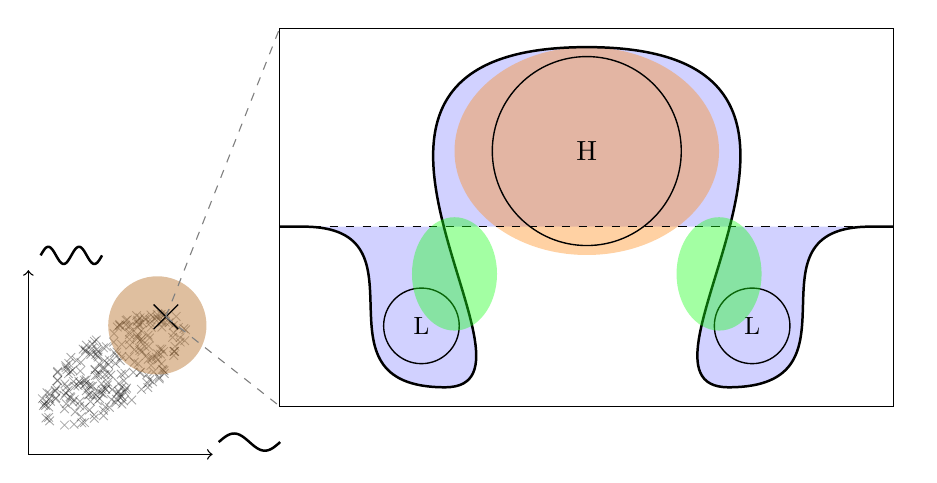
\begin{tikzpicture}[scale=1.2]
      \def\smallcross#1#2#3{%
    \draw[line width=0.3pt,black,opacity=#3]
      (#1,#2) ++(-0.035,-0.035) -- ++(0.07,0.07)
      (#1,#2) ++(-0.035,0.035) -- ++(0.07,-0.07);%
  }
\draw[line width=0.3pt] (-3.25,-1.9) rectangle (3.25,2.1);
\fill[blue!60,opacity=.3,even odd rule]
    (-3,0)
    .. controls (-1.6,0) and (-3.0,-1.7) ..
    (-1.5,-1.7)
    .. controls (-0.2,-1.7) and (-3.4,1.9) ..
    (0,1.9)
    .. controls (3.4,1.9) and (0.2,-1.7) ..
    (1.5,-1.7)
    .. controls (3.0,-1.7) and (1.6,0) ..
    (3,0)
    -- cycle;

\fill[orange!90,opacity=.4] (0,.8) ellipse (1.4 and 1.1);

\draw[dashed] (-3.25,0) -- (3.25,0);

\draw[line width=0.9pt]
    (-3.25,0)
    -- (-3,0)
    .. controls (-1.6,0) and (-3.0,-1.7) ..
    (-1.5,-1.7)
    .. controls (-0.2,-1.7) and (-3.4,1.9) ..
    (0,1.9)
    .. controls (3.4,1.9) and (0.2,-1.7) ..
    (1.5,-1.7)
    .. controls (3.0,-1.7) and (1.6,0) ..
    (3,0)
    -- (3.25,0);

\draw[line width=0.5pt] (0,.8) circle (1.) node {H};
\draw[line width=0.5pt] (-1.75,-1.05) circle (0.4) node {\small L};
\draw[line width=0.5pt] (1.75,-1.05) circle (0.4) node {\small L};

\fill[green!90,opacity=.4]
    (-1.4,-0.5) ellipse (0.45 and 0.6);
\fill[green!90,opacity=.4,]
    (1.4,-0.5) ellipse (0.45 and 0.6);

% \begin{scope}[shift={(3.5,1.5)},scale=1.2]
\begin{scope}[shift={(-5,-1.5)}, scale=1.3]
    \pgfmathsetseed{7}
    \begin{scope}
        % \clip (0.02,0.02) rectangle (0.7,0.7);
        \foreach \i in {1,...,250}{
            \pgfmathsetmacro{\th}{360*rnd}
            \pgfmathsetmacro{\rr}{sqrt(rnd)}
            \pgfmathsetmacro{\px}{0.7*\rr*cos(\th)}
            \pgfmathsetmacro{\py}{0.30*\rr*sin(\th)}
            \pgfmathsetmacro{\cx}{\px*cos(35)-\py*sin(35)}
            \pgfmathsetmacro{\cy}{\px*sin(35)+\py*cos(35)}
            \smallcross{\cx}{\cy}{0.35}
        }
    \end{scope}
    \fill[brown,opacity=.5] (0.35,0.35) circle (0.4);
    \draw[line width=0.5pt,->] (-0.7,-0.7) -- (0.8,-0.7);
    \draw[line width=0.5pt,->] (-0.7,-0.7) -- (-0.7,0.8);
    \coordinate (blackcross) at (0.42,0.42);
    \draw[line width=0.5pt] (blackcross) ++(-0.1,-0.1) -- ++(0.2,0.2);
    \draw[line width=0.5pt] (blackcross) ++(-0.1,0.1) -- ++(0.2,-0.2);
        % \draw[line width=0.9pt] (-0.6,-0.6) -- (-0.2,-0.6);
    \draw[line width=0.9pt,domain=0:360,samples=60,smooth]
        plot ({0.85+\x/360*0.5},{-0.6 + 0.07*sin(\x)});
    \draw[line width=0.9pt,domain=0:720,samples=90,smooth]
        plot ({-0.6+\x/720*0.5},{0.92+0.07*sin(\x)});
\end{scope}

\draw[dashed,gray] (blackcross) -- (-3.25,-1.9);   % to bottom-left corner
\draw[dashed,gray] (blackcross) -- (-3.25,2.1);    % to top-left corner

\end{tikzpicture}
\end{document}